\documentclass[a4paper]{article}
\usepackage{header}

\usepackage{tikz}
\usepackage{tikz-network}
\usepackage{float}

\newcommand\enumtocitem[3]{\item\textbf{#1}\addtocounter{#2}{1}\addcontentsline{toc}{#2}{\protect{\numberline{#3}} #1}}
\newcommand\defitem[1]{\enumtocitem{#1}{subsection}{\thesubsection}}
\newcommand\proofitem[1]{\enumtocitem{#1}{subsection}{\thesubsection}}

\newlist{colloq}{enumerate}{1}
\setlist[colloq]{leftmargin=*,label=\textbf{\arabic*.}}

\newtheoremstyle{named}{}{}{}{}{\bfseries}{}{.5em}{Теорема \thmnote{#3}}
\theoremstyle{named}
\newtheorem*{namedtheorem}{Theorem}

\graphicspath{
    {img/}
}

\renewcommand{\gcd}{\text{НОД}}
\renewcommand{\O}{\text{O}}
\newcommand{\E}{\text{E}}
\DeclareMathOperator{\MAJ}{\mathrm{MAJ}}


\title{\HugeДискретная математика, Коллоквиум 2}
\author{
	Балюк Игорь \\
	\href{https://teleg.run/lodthe}{@lodthe},
    \href{https://github.com/LoDThe/hse-tex}{GitHub} \\
}

\usepackage[yyyymmdd,hhmmss]{datetime}
\settimeformat{xxivtime}
\renewcommand{\dateseparator}{.}
\date{Дата изменения: \today \ в \currenttime}

\begin{document}
    \maketitle

    Материалы взяты из учебника Александра Рубцова.

    \tableofcontents

    \newpage

    \section{Определения}

    Контрольный вопрос на понимание определений включает в себя формулировку одного определения из списка ниже и контрольный вопрос по этому определению. Пример: <<Определение полного прообраза. Пусть $f(x) = x^2$ --- функция из $\ZZ$ в $\ZZ$. Найдите полный прообраз множества $\{1, 2, 3, 4\}$.

    \begin{colloq}
    
    \defitem{Деление целых чисел с остатком.}

        Говорят, что целое число $a$ делится на целое число $b$, если $a = bk$ для некоторого целого числа $k$. В этом случае говорят также <<$a$ кратно $b$>>, и <<$b$ является делителем числа $a$>>.

        Теперь определим деление с остатком. Пусть $b$ --- целое положительное число. Деля на $b$ с остатком, мы связываем  предметы в пачки по $b$ в каждой, пока это возможно: количество полных пачек называется частным (говорят ещё <<неполное частное>>, чтобы отличать от частного как дроби), и сколько-то предметов останется, их количество и называют остатком.

        Формально: разделить целое $a$ на целое положительное $b$ означает найти такое целое $q$ (\textit{частное}) и такое $r$ (\textit{остаток}), что
        \begin{equation*}
            a = b \cdot q + r; \quad 0 \leq r < b.
        \end{equation*}


    \defitem{Сравнения по модулю. Основные свойства.}

        Если два числа $a$ и $b$ дают одинаковые остатки при делении на положительное число $N$, то говорят, что они \textit{сравнимы} по модулю $N$, и пишут $a \equiv b \pmod N$.

        Эквивалентное определение: $a$ и $b$ сравнимы по модулю $N$, если разность $a - b$ делится на $N$.

        Рассмотрим основные свойства:
        \begin{enumerate}
        \item $a \equiv b \pmod c \iff b \equiv a \pmod c$

        \item $a \equiv b \pmod c \iff (a - x) \equiv (b - x) \pmod c$

        \item $x \equiv a \pmod m, y \equiv b \pmod m \implies xy \equiv ab \pmod m$

        \item $a \equiv 0 \pmod c \iff c \mid a$

        \item $a \equiv b \pmod d, b \equiv c \pmod d \iff a \equiv c \pmod d$
        \end{enumerate}
        
        Например, можно найти $2^{100} \bmod 7$ (остаток от деления $2^{100}$ на $7$): поскольку $2^3 = 8 \equiv 1 \pmod 7$, то $2^{99} = (2^{3})^{33} \equiv 1^{33} = 1 \pmod 7$, так что $2^{100} = 2^{99} \cdot 2 \equiv 1 \cdot 2 = 2 \pmod 7$.

    \defitem{Арифметика остатков (вычетов). Обратимые остатки (вычеты).}

        Остаток (вычет) по модулю $N$ называется \textbf{обратимым}, если в произведении с каким-то другим остатком он даёт $1$. Другими словами, $a$ обратим, если уравнение $a \cdot x \equiv 1 \pmod N$ имеет решение.

    \defitem{Малая теорема Ферма.}

        \begin{theorem*}
            Если $p$ --- простое число, то
            \begin{equation*}
                a^{p - 1} \equiv 1 \pmod p
            \end{equation*}
            при любом $a$, не делящемся на $p$.
        \end{theorem*}

    \defitem{Функция Эйлера. Теорема Эйлера.}

        \begin{theorem*}
            Пусть $N > 1$ --- произвольное целое число, а $\phi(N)$ равно количеству остатков среди $0, 1, \dots, N - 1$, взаимно простых с $N$. Пусть $a$ --- один из этих остатков. Тогда
            \begin{equation*}
                a^{\phi(N)} \equiv 1 \pmod N.
            \end{equation*}
        \end{theorem*}

        Функцию $\phi$ называют \textbf{функцией Эйлера} и традиционно обозначают буквой $\phi$.  Если $N$ простое, то $\phi(N) = N - 1$, и теорема Эйлера превращается в малую теорему Ферма.

    \defitem{Наибольший общий делитель. Алгоритм Евклида.}

        Наибольшим общим делителем ($\gcd$) для двух целых чисел $m$ и $n$ называется наибольший из их общих делителей. Пример: для чисел $54$ и $24$ наибольший общий делитель равен $6$.

        Алгоритм Евклида помогает найти $\gcd$ двух целых чисел.

        \begin{itemize}
        \item \textbf{Геометрическая интерпретация}.
            Пусть даны два отрезка длины $a$ и $b$. Вычтем из большего отрезка меньший и заменим больший отрезок полученной разностью. Повторяем эту операцию, пока отрезки не станут равны. Если это произойдёт, то исходные отрезки соизмеримы, и последний полученный отрезок есть их наибольшая общая мера. Если общей меры нет, то процесс бесконечен и отрезки несоизмеримы.

        \item \textbf{Алгебраическая интерпретация}.
            Пусть нам даны два целых числа $a$ и $b$. Вычтем из большего числа меньшее и заменим большее на полученную разность. Повторяем эту операцию, пока числа не станут равны. Последнее полученное число будет их наибольшим общим делителем. Это можно записать в виде следующей системы:
            \begin{equation*}
                \begin{cases}
                    a_0 = q_1 \cdot a_1 + a_2 \\
                    a_1 = q_2 \cdot a_2 + a_3 \\
                    \vdots \\
                    a_{k - 2} = q_{k - 1} \cdot a_{k - 1} + a_k \\
                    a_{k - 1} = q_k \cdot a_k.
                \end{cases}
            \end{equation*}

            Тогда $q_k = \text{\gcd}(a_0, a_1)$.

        \end{itemize}

        Алгоритм можно ускорить с помощью деления:
        \begin{enumerate}
            \item
                Большее число делим на меньшее.
            \item
                Если делится без остатка, то меньшее число и есть $\gcd$ (следует выйти из цикла).
            \item
                Если есть остаток, то большее число заменяем на остаток от деления.
            \item
                Переходим к пункту 1.
        \end{enumerate}

    \defitem{Расширенный алгоритм Евклида нахождения решения линейного диофантова уравнения.}

        \textit{Линейное диофантово уравнение} --- уравнение вида $ax + by = c$. Решить диофантово уравнение означает найти все такие целые $x$, $y$, чтобы выполнялось равенство.

        Если c делится на $\gcd(a, b)$, диофантово уравнение имеет бесконечно много решений. В противном случае, оно не имеет решений вообще.
        
        Если $x_0$, $y_0$ --- какое-то частное решение диофантова уравнения, то тогда общее решение выражается следующим образом:
        \begin{equation*}
            \begin{cases}
                x = x_0 + k \cdot \dfrac{b}{\gcd(a, b)}, &k \in \ZZ, \\
                y = y_0 - k \cdot \dfrac{a}{\gcd(a, b)}, &k \in \ZZ, \\
            \end{cases}
        \end{equation*}

        \textbf{Расширенный алгоритм Евклида} --- алгоритм, который находит $\gcd$ двух чисел и коэффициенты, с помощью которых он выражается через эти числа, то есть такие $x$, $y$, что $ax + by = \gcd(a, b)$. Чтобы получить решение диофантова уравнения, можно домножить $x$ и $y$ на $\dfrac{c}{\gcd(a, b)}$.

        Расширенный алгоритм Евклида представляет собой применение обычного алгоритма Евклида, а потом прохода <<обратно>>, пользуясь следующим свойством: если пара $(x_1, y_1)$ является решением уравнения $(b \bmod a) \cdot x_1 + a \cdot y_1 = \gcd(a, b)$, то пара $(x, y)$, такая что
        \begin{equation*}
            \begin{cases}
                x = y_1 - \floor*{\dfrac{b}{a}} \cdot x_1 \\
                y = x_1 \\
            \end{cases}
        \end{equation*}
        является решением уравнения $ax + by = \gcd(a, b)$. 

        Тем самым, надо выполнять алгоритм Евклида для чисел $(a, b)$, а потом восстановить все предыдущие $(x_k, y_k)$ зная $(x_{k + 1}, y_{k + 1})$.

    \defitem{Простые числа, формулировка основной теоремы арифметики.}
 
        Целое число $p > 1$ называется простым, если оно не разлагается в произведение меньших чисел (то есть не имеет положительных делителей, кроме $1$ и $p$).

        \begin{theorem*}
            Всякое целое положительное число, большее $1$, разлагается на простые множители, причём единственным образом: любые два разложения отличаются только перестановкой сомножителей.
        \end{theorem*}

    \defitem{Равномощные множества.}

        Множество $A$ называется равномощным множеству $B$, если существует биекция из множества $A$ в множество $B$.

    \defitem{Cчётные множества.}

        Множество называется счётным, если оно равномощно множеству натуральных чисел $\NN$.

    \defitem{Множества мощности континуум.}

        Множество имеет мощность \textbf{континуум}, если оно равномощно $\RR$.

    \defitem{Основные определения элементарной теории вероятностей: исходы, события, вероятность события.}

        \textbf{Вероятностным пространством} называется конечное множество $U$, его элементы называются \textbf{возможными исходами}. \textbf{Событием} называется произвольное подмножество $A \subseteq U$. 

        На вероятностном пространстве задана функция $Pr: U \to [0; 1]$, такая что $\sum_{x \in U} \Pr[x] = 1$. Функция $Pr$ называется \textbf{вероятностным распределением}, а число $Pr[x]$ называется \textbf{вероятностью исхода} $x \in U$. Вероятностью события $A$ называется число $Pr[A] = \sum_{x \in A} \Pr[x]$.

    \defitem{Формулировка формулы включений и исключений для вероятностей.}

        Для всякой вероятностной модели и для произвольных множеств $A_1, \dots, A_n \subseteq U$ верно
        \begin{equation*}
            \Pr[A_1 \cup A_2 \cup \dots \cup A_n] = \sum_i \Pr[A_i] - \sum_{i < j} \Pr[A_i \cap A_j] + \dots = \sum_{\varnothing \neq I \subseteq \{1, 2, \dots, n\}} (-1)^{|I| + 1} Pr\left[\bigcap_{i \in I} A_i\right].
        \end{equation*}

    \defitem{Условная вероятность.}

        Помимо вероятностей тех или иных событий бывает нужным говорить и о вероятностях одних событий при условии других. Неформально говоря, мы хотим определить вероятность выполнения события $A$ в том случае, когда событие $B$ выполняется. 
        
        В терминах вероятностного пространства определение этого понятия довольно естественное: нужно сузить вероятностное пространство на множество $B$. Так, для равновозможной модели мы получаем, что вероятность $A$ при условии $B$ есть просто $\dfrac{|A \cap B|}{|B|}$, то есть число благоприятных исходов поделенное на число всех исходов (после сужения всего вероятностного пространства до $B$). 
        
        В случае произвольного вероятностного пространства нужно учесть веса исходов, то есть нужно сложить вероятности исходов в $A \cap B$ и поделить на сумму вероятностей исходов в $B$.

        Таким образом, мы приходим к формальному определению. \textbf{Условной вероятностью} события $A$ при условии $B$ называется число
        \begin{equation*}
            \Pr[A \mid B] = \dfrac{Pr[A \cap B]}{\Pr[B]}.
        \end{equation*}


    \defitem{Независимые события. Основные свойства независимых событий.}

        События $A$ и $B$ называются независимыми, если
        \begin{equation*}
            \Pr[A] = \Pr[A \mid B].
        \end{equation*}

        Из определения условной вероятности мы сразу получаем эквивалентное определение независимостей событий. Событие $A$ не зависит от события $B$, если
        \begin{equation*}
            \Pr[A \cap B] = \Pr[A] \cdot \Pr[B].
        \end{equation*}

    \defitem{Формула полной вероятности.}

        \begin{lemma*}
            Пусть $B_1, B_2, \dots, B_n$ --- разбиение вероятностного пространства, то есть $U = B_1 \cup B_2 \cup \dots \cup B_n$, где $B_i \cap B_j = \varnothing$ при $i \neq j$. Пусть также $Pr[B_i] > 0$ для всякого $i$. Тогда для всякого события $A$
            \begin{equation*}
                \Pr[A] = \sum_{i = 1}^n \Pr[A \mid B_i] \cdot \Pr[B_i].
            \end{equation*}
        \end{lemma*}

    \defitem{Случайная величина и математическое ожидание. Линейность математического ожидания.}

        \textbf{Случайная величина} --- это числовая функция на вероятностном пространстве, то есть функция вида $\xi: U \to \RR$. То есть, по сути, случайная величина --- это обычная числовая функция, но теперь на её аргументах задано вероятностное распределение.

        \textbf{Математическим ожиданием} случайной величины $\xi: U \to \RR$ называется число
        \begin{equation*}
            \E[\xi] = \sum_{u \in U} \xi(u) \cdot \Pr[u]
        \end{equation*}

        \begin{lemma*} (линейность математического ожидания) 
            Пусть $\xi: U \to \RR$ и $g: U \to \RR$ --- две случайные величины на одном и том же вероятностном пространстве. Тогда
            \begin{equation*}
                \E[f + g] = \E[f] + \E[g].
            \end{equation*}
        \end{lemma*}

    \defitem{Формулировка неравенства Маркова.}

        \begin{namedtheorem}[(Неравенство Маркова)]
            Пусть $\xi$ --- случайная величина, принимающая только \textbf{неотрицательные} значения. Тогда для всякого $x > 0$ верно
            \begin{equation*}
                \Pr[\xi \geq x] \leq \dfrac{\E[\xi]}{x}.
            \end{equation*}
        \end{namedtheorem}

        То есть, вероятность того, что случайная величина $\xi$ сильно больше своего математического ожидания, не слишком велика (заметим, что лемма становится содержательной, когда $x > \E[\xi]$).

    \defitem{Определение схемы в некотором функциональном базисе. Представление схем графами.}

        \textbf{Полным базисом} называется набор связок, если через эти связки выражается любая булева функция.

        \textbf{Стандартным базисом} назовём набор из операций конъюнкция (И), дизъюнкция (ИЛИ) и отрицание (НЕ). 

        \textbf{Булевой схемой} от переменных $x_1, \dots, x_n$ мы будем называть последовательность булевых функций $g_1, \dots, g_s$, в которой всякая $g_i$ получается из предыдущих функций последовательности и переменных применением одной из логических операций из выбранного базиса для этой схемы.

        В булевой схеме задано некое число $m \geq 1$ и члены последовательности $g_{s - m + 1}, \dots, g_s$ называются \textbf{выходами схемы}. Число $m$ называют числом выходов схемы.

        Мы говорим, что схема вычисляет булеву функцию $f: \{0, 1\}^n \to \{0, 1\}^m$, если для всякого $x \in \{0, 1\}^n$ верно $f(x) = (g_{s - m + 1}(x), \dots, g_{s}(x))$.

        \textbf{Размером} схемы называют число $s$.

        Рассмотрим представление схемы графом:
        \begin{figure}[H]
            \caption{Схема функции $x_1 \oplus x_2$}
            \centering
            \begin{tikzpicture}
                \Vertex[y=0,x=0,label=$x_1$]{x1}
                \Vertex[y=2,x=0,label=$x_2$]{x2}
                \Vertex[y=0,x=1.5,label=$\neg$]{nx1}
                \Vertex[y=2,x=1.5,label=$\neg$]{nx2}
                \Vertex[y=0,x=3,label=$\land$]{ax1}
                \Vertex[y=2,x=3,label=$\land$]{ax2}
                \Vertex[y=1,x=4.5,label=$\lor$]{end}
                \Edge[Direct](x1)(nx1)
                \Edge[Direct](x2)(nx2)
                \Edge[Direct](nx1)(ax1)
                \Edge[Direct](x2)(ax1)
                \Edge[Direct](nx2)(ax2)
                \Edge[Direct](x1)(ax2)
                \Edge[Direct](ax1)(end)
                \Edge[Direct](ax2)(end)
            \end{tikzpicture}
        \end{figure}

    \defitem{Полный базис. Примеры полных и неполных базисов.}

        \textbf{Полным базисом} называется набор связок, если через эти связки выражается любая булева функция.

        \textbf{Стандартным базисом} назовём набор из операций конъюнкция (И), дизъюнкция (ИЛИ) и отрицание (НЕ).

        Примеры полных базисов:
        \begin{enumerate}
        \item Базис $\{\land, \lor, \neg\}$ полный, так как всякую булеву функцию можно выразить через ДНФ.

        \item Базис $\{\neg, \land\}$ полный, так как $x_1 \lor x_2 = \neg(\neg x_1 \land \neg x_2)$.

        \item Базис $\{\neg, \lor\}$ полный, так как $x_1 \land x_2 = \neg(\neg x_1 \lor \neg x_2)$.

        \item Базис $\{\mid\}$ (штрих Шеффера) полный, так как $\neg x = x \mid x$ и $x_1 \land x_2 = \neg(x_1 \mid x_2) = (x_1 \mid x_2) \mid (x_1 \mid x_2)$.

        \item Базис $\{1, \oplus, \land\}$ полный, так как всякую булеву функцию можно выразить многочленом Жегалкина.
        \end{enumerate}

        Примеры неполных базисов:
        \begin{enumerate}
            \item Базис $\{\land, \lor\}$ неполный, так как он монотонный.

            \item Базис $\{\oplus, \land\}$.

            \item Базис $\{\lor, \to\}$.
        \end{enumerate}

    \defitem{Полином Жегалкина (в стандартном виде).}

        \textbf{Многочленом Жегалкина} называется формула вида
        \begin{equation*}
            \bigoplus_{S \subseteq \{1, \dots, n\}} a_S \bigwedge_{i \in S} x_i, \quad a_S \in \{0, 1\}.
        \end{equation*}

        Примеры многочлена Жегалкина:
        \[\begin{gathered}
            1 \oplus x_1 \oplus x_2 \oplus x_3 \oplus (x_1 \land x_2) \oplus (x_1 \land x_3) \oplus (x_2 \land x_3) \oplus (x_1 \land x_2 \land x_3); \\
            x_3 \oplus (x_1 \land x_3) \oplus (x_2 \land x_3) \oplus (x_1 \land x_2 \land x_3).
        \end{gathered}\]

        Для простоты чтения $\land$ можно опускать:
        \begin{equation*}
            1 \oplus x_1 \oplus x_2 \oplus x_3 \oplus x_1 x_2 \oplus x_1 x_3 \oplus x_2 x_3 \oplus x_1 x_2 x_3; \\
        \end{equation*}

    \defitem{Схемная сложность функции (размер схемы).}

        \textbf{Схемная сложность} булева отображения $f: \{0, 1\}^n \to \{0, 1\}^m$ (в частности, булевой функции) --- это наименьший размер (количество присваиваний) схемы, вычисляющей это выражение.

    \end{colloq}

    \section{Задачи}

    На коллоквиуме Вам может попасться похожая по уровню задача не из этого списка.

    \begin{colloq}

    \defitem{Приведите пример таких целых чисел $a$, $b$, $c$, что $\gcd(ab, c) \neq \gcd(a, c) \cdot \gcd(b, c$.}
    \defitem{На сколько нулей заканчивается число $16!$?}
    \defitem{Найдите остаток от деления $2^{38}$ на $37$.}
    \defitem{Решите диофантово уравнение $12x + 19y = 7$.}
    \defitem{Сколько есть положительных целых делителей у числа $66^{66}$?}
    \defitem{Вероятностное пространство: последовательности $(x_1 , x_2, x_3 , x_4)$ длины $4$, состоящие из целых чисел в диапазоне от $1$ до $6$. Все исходы равновозможны. Найдите вероятность события <<$\overline{x_1 x_2 x_3 x_4}$ чётно>>.}
    \defitem{Приведите пример вероятностного пространства и таких событий $A$, $B$ в этом пространстве, что $\Pr[A \mid B] = \frac{1}{3} \Pr[A]$.}
    \defitem{Существуют ли такие события $A$ и $B$, что $\Pr[A] = \Pr[B] = \Pr[A \mid B] = 1/2$, а $\Pr[B \mid A] = 1/3$?}
    \defitem{О событиях $A$ и $B$ вероятностного пространства $U$ известно, что $\Pr[A] = Pr[B] = 4/5$. Могут ли при этом события $A \cup B$ и $B$ быть независимыми?}
    \defitem{Про неотрицательную случайную величину $\xi$ известно, что $Pr[\xi > 10] < 1/4$. Найдите возможные значения математического ожидания $\E[\xi]$.}
    \defitem{Вероятностное пространство: последовательности $(x_1 , x_2, x_3 , x_4)$ длины $4$, состоящие из целых чисел в диапазоне от $1$ до $6$. Все исходы равновозможны. Найдите математическое ожидание случайной величины $x_1 + x_2 + x_3 + x_4$.}
    \defitem{По $15$ мальчиков и девочек стоят в шеренге в случайном порядке. Сколько в среднем девочек стоит левее всех мальчиков?}
    \defitem{Докажите, что множество непересекающихся отрезков на прямой конечно или счетно.}
    \defitem{Докажите, что всякое бесконечное множество содержит бесконечное число непересекающихся счет-
    ных подмножеств.}
    \defitem{Докажите, что биекций на множестве натуральных чисел континуум.}
    \defitem{Постройте ДНФ и КНФ разложения для булевой функции, заданной вектором значений $10100110$.}
    \defitem{Является ли полным базис, состоящий из функций $x_1 \oplus x_2 \oplus x_3$, $x_1 x_2$, $1$.}
    \defitem{Найдите полином Жегалкина для функции $\MAJ_4(x, y, z, t)$.}
    \defitem{Рассматриваем схемы в стандартном базисе. Пусть схемная сложность функции $f$ не больше $A$,
    а схемная сложность функции $g$ не больше $B$. Докажите, что схемная сложность функции $f \oplus g$ не больше $A + B + 5$.}
    \defitem{Постройте схему полиномиального размера, вычисляющую функцию $\MAJ_n$.}

    \end{colloq}

    \section{Вопросы на знание доказательств}
    \begin{colloq}
    \setlength\parindent{20pt}

    \proofitem{Сравнение $ax \equiv 1 \pmod{N}$ имеет решение тогда и только тогда, когда $\text{НОД}(a, N) = 1$.}

        \begin{theorem*}
            Сравнение $ax \equiv 1 \pmod N$ имеет решение тогда и только тогда, когда $\gcd(a, N) = 1$.
        \end{theorem*}

        \begin{proof}
            Докажем теорему в обе стороны.
            \begin{itemize}
            \item $\Leftarrow$: 
                Пусть $\gcd(a, N) = 1$. Следовательно, $\exists k_1, k_2 : k_1 a + k_2 N = 1$ (следует из алгоритма Евклида). Вычислим остаток при делении на $N$ обеих частей:
                \[\begin{gathered}
                    \begin{cases}
                        k_1 a + k_2 N &\equiv k_1 a \pmod N \\
                        1 &\equiv 1 \pmod N
                    \end{cases} \\
                    \Downarrow \\
                    k_1 a \equiv 1 \pmod N.
                \end{gathered}\]

                Следовательно, $k_1$ и есть искомый $x$, при котором $ax \equiv 1 \pmod N$.

            \item $\Rightarrow$:
                Пусть $\exists x : ax \equiv 1 \pmod N$. Тогда $\exists t : ax - tN = 1$. Требуется доказать, что в этом случае $\gcd(a, N) = 1$. Докажем от противного.

                Пусть $\gcd(a, N) = d > 1$. Тогда $\exists k_1, k_2 : a = k_1 d$ и $N = k_2 d$. Подставим эти произведения в выражение
                \begin{equation*}
                    k_1 d x - k_2  d t = 1 \implies d (k_1 x - k_2 t) = 1.
                \end{equation*}

                Это возможно только при $d = 1$. Следовательно, $\gcd(a, N) = 1$.
            \end{itemize}
        \end{proof}

    \proofitem{Малая теорема Ферма.}

        \begin{theorem*}
            Если $p$ --- простое число, то
            \begin{equation*}
                a^{p - 1} \equiv 1 \pmod p
            \end{equation*}
            при любом $a$, не делящемся на $p$.
        \end{theorem*}

        \begin{proof}~

            Сначала докажем нужную для доказательства лемму.

            \begin{lemma*}
                Если вычислить остатки по модулю $p$ от $a, 2a, \dots, (p - 1) \cdot a$, то получатся остатки $1, 2, \dots, p - 1$ в некотором порядке.
            \end{lemma*}

            \begin{proof}
                Докажем от противного. Пусть нашлись каких-то два числа $ax$ и $ay$, дающих одинаковый остаток при делении на $p$ ($x$, $y$ --- остатки). Тогда $a \cdot (x - y)$ делится на $p$, что невозможно (так как $a$ не делится на $p$). Тогда нет совпадающих остатков, так как произведений и остатков $p - 1$.
            \end{proof}

            Рассмотрим произведение $a, 2a, 3a, \dots, (p - 1)a$. Тогда
            \begin{equation*}
                a \cdot 2a \cdot \dots \cdot (p - 1) a \equiv a^{p - 1} \cdot (p - 1)! \pmod p.
            \end{equation*}

            С другой стороны, по лемме это эквивалентно $(p - 1)!$ по модулю $p$ (произведение остатков в другом порядке). Тогда $a^{p - 1} \equiv 1 \pmod p$, что и требовалось доказать.
        \end{proof}

    \proofitem{Теорема Эйлера.}

        \begin{theorem*}
            Пусть $n > 1$ --- произвольное целое число, а $\phi(N)$ равно количеству остатков среди $0, 1, \dots, n - 1$, взаимно простых с $n$. Пусть $a$ --- один из этих остатков. Тогда
            \begin{equation*}
                a^{\phi(n)} \equiv 1 \pmod n.
            \end{equation*}
        \end{theorem*}

        \begin{proof}
            Заметим, что достаточно рассматривать остаток от деления $a$ на $n$.

            Рассмотрим граф, где каждой вершине соответствует какой-то остаток, взаимно простой с $n$, а ребром из $x$ в $y$ будем называть преобразование $x \to y$. Тогда в графе будет $\phi(n)$ вершин. Так как $a$ взаимно просто с $n$, то
            \begin{itemize}
            \item
                Для каждой вершины графа $x$ получаем, что $ax$ взаимно просто с $n$ (так как $x$ взаимно просто с $n$ по построению). Из этого следует, что всегда возможно провести ребро $x \to ax$, если его нет.

            \item
                Уравнение $ax \equiv b \pmod n$ имеет единственное решение (по модулю $n$) для любого $b$. Из этого следует, что из каждой вершины графа выходит ровно одно ребро и в каждую вершину входит ровно одно ребро.
            \end{itemize}

            Тогда граф обязан разбиться на циклы, так как иначе процесс умножения можно продолжать сколь угодно долго и условие на количество ребер нарушится. 
            
            Пусть $k$ --- степень такая, что $a^k \equiv 1 \pmod n$. Заметим, что она существует, так как для единицы существует цикл:
            \begin{equation*}
                1 \to a \to a^2 \to \dots \to a^k.
            \end{equation*}

            Докажем, что все циклы имеют одинаковую длину. Очевидно, что длину, большую $k$ цикл иметь не может (так как $b \cdot a^k \equiv b \pmod n$ и цикл замкнётся). Пусть для какого-то $b$ есть цикл длины $l < k$.

            Тогда $b \cdot a^l \equiv b \pmod n$ и (так как $b$ взаимно просто с $n$, то у него есть обратный элемент) $a^l \equiv 1 \pmod n$.

            Приходим к противоречию. Тогда $\phi(n) = km$ для какого-то $m$ и
            \begin{equation*}
                a^{\phi(n)} \equiv a^{km} \equiv 1^m = 1 \pmod n,
            \end{equation*}
            что и требовалось доказать.
        \end{proof}

    \proofitem{Корректность алгоритма Евклида и расширенного алгоритма Евклида.}

        \begin{namedtheorem}[(Алгоритм Евклида)]
            Пусть $a$, $b$ --- целые числа, не равные одновременно нулю. Определим последовательность чисел:
            \begin{equation*}
                a \geq b > r_1 > r_2 > \dots > r_n,
            \end{equation*}
            где $\forall k : r_k$ --- это остаток от деления $r_{k - 2}$ на $r_{k - 1}$. Тогда $\gcd(a, b)$ равен последнему ненулевому члену этой последовательности, то есть $r_n$.
        \end{namedtheorem}

        \begin{proof}
            Пусть $a = b \cdot q + r$. Тогда требуется доказать, что $\gcd(a, b) = \gcd(b, r)$:
            \begin{enumerate}
            \item
                Пусть $d$ --- любой общий делитель чисел $a$ и $b$, необязательно наибольший, тогда $a = t_1 \cdot d$ и $b = t_2 \cdot d$, где $t_1$, $t_2$ --- целые числа.

            \item
                Тогда $d$ также является общим делителем чисел $b$ и $r$, так как $b$ делится на $d$ по определению, а $r = a - b \cdot q = t_1 \cdot d - t_2 \cdot d \cdot q = d \cdot (t_1 - t_2 \cdot q)$.

            \item
                Верно и обратное: пусть $d$ --- общий делитель $b$ и $r$, то есть $b = t_2 \cdot d$ и $r = t_3 \cdot d$. Тогда $b$ делится на $d$ по определению, и $a = q \cdot b + r = q \cdot t_2 \cdot d + t_3 \cdot d = d \cdot (q \cdot t_2 + t_3)$.

            \item
                Следовательно, все общие делители пар чисел $(a, b)$ и $(b, r)$ совпадают. В частности, совпадает и наибольший общий делитель.
            \end{enumerate}

            Алгоритм конечный, так как за одну итерацию одно из чисел становится меньше своего предыдущего значения, причем могут получаться только неотрицательные числа.
        \end{proof}

        \begin{namedtheorem}[(Расширенный алгоритм Евклида)]
            Пусть $a$, $b$ --- целые числа, $d = \gcd(a, b)$. Тогда существуют $x$, $y$, такие что $ax + by = d$.
        \end{namedtheorem}

        \begin{proof}~
            
            \begin{enumerate}
            \item
                Пусть $a = b \cdot q + r$. Из доказательства алгоритма Евклида известно, что $\gcd(a, b) = \gcd(b, r)$. Воспользуемся этим свойством, чтобы найти $x$ и $y$.

            \item
                Пусть $x'$ и $y'$ --- числа, такие что $bx' + ry' = \gcd(a, b)$. Заметим, что $r$ можно выразить с помощью арифметических операций через $a$ и $b$:
                \begin{equation*}
                    r = a - \floor*{\dfrac{a}{b}} \cdot b.
                \end{equation*}

            \item
                Подставим полученное в уравнение:
                \begin{equation*}
                    bx' + ry' = bx' + \left(a - \floor*{\dfrac{a}{b}} \cdot b\right) \cdot y' = bx' + ay' - \floor*{\dfrac{a}{b}} \cdot b \cdot y' = ay' + b \cdot \left(x' - \floor*{\dfrac{a}{b}} \cdot y'\right).
                \end{equation*}

            \item
                С одной стороны: $\gcd(a, b) = ay' + b \cdot \left(x' - \floor*{\dfrac{a}{b}} \cdot y'\right)$.

                С другой стороны: $\gcd(a, b) = ax + by$. Отсюда получаем, что $x = y'$ и $y = x' - \floor*{\dfrac{a}{b}} \cdot y'$.

            \item
                Таким образом, зная $x'$ и $y'$, такие что $bx' + ry' = \gcd(a, b)$, можно на каждом шаге алгоритма Евклида получить $x$ и $y$, такие что $ax + by = \gcd(a, b)$.

                Для случая, когда $r = 0$, разложение очевидно: $x' = 1, y' = 0$. Из него можно получить остальные коэффициенты.
            \end{enumerate}
        \end{proof}

    \proofitem{Основная теорема арифметики.}

        \begin{theorem*}
            Всякое целое положительное число, большее $1$, разлагается на простые множители, причём единственным образом: любые два разложения отличаются только перестановкой сомножителей.
        \end{theorem*}

        \begin{proof}~

            \begin{itemize}
            \item \textbf{Существование}.
                Докажем существование разложения числа $n$ на простые множители, предполагая, что оно уже доказано для любого другого числа, меньшего $n$. Если $n$ --- простое, то существование доказано. Если $n$ --- составное, то оно может быть представлено в виде произведения двух чисел $a$ и $b$, каждое из которых больше $1$, но меньше $n$. Числа $a$ и $b$ либо являются простыми, либо могут быть разложены в произведение простых (уже доказано ранее). Подставив их разложение в $n = a \cdot b$, получим разложение исходного числа $n$ на простые.

            \item \textbf{Единственность}.
                Пусть некоторое число $N$ имеет два разложения:
                \begin{equation*}
                    N = p_1 \cdot p_2 \cdot \dots \cdot p_n = q_1 \cdot q_2 \cdot \dots \cdot q_m.
                \end{equation*}

                Сократим общие сомножители, если они есть. Если сократится не всё, то получим два разложения одного числа, не имеющих общих сомножителей (для удобства оставим $n$ и $m$):
                \begin{equation*}
                    p_1 \cdot p_2 \cdot \dots \cdot p_n = q_1 \cdot q_2 \cdot \dots \cdot q_m.
                \end{equation*}

                Докажем следующее утверждение: если $p$ --- простое число, то произведение чисел, каждое из которых не делится на $p$, не может делиться на $p$. Действительно, если $a \not\equiv 0 \pmod p$ и $b \not\equiv 0 \pmod p$, то и $a \cdot b \not\equiv 0 \pmod p$.

                Правая часть равенства выше --- это произведение чисел, каждое из которых не делится на $p_1$, следовательно, все произведение не делится на $p_1$. Приходим к противоречию, когда $q_1 \cdot \dots \cdot q_m = n$, но $n \not\equiv 0 \pmod{p_1}$. Следовательно, разложение числа $N$ на простые множители единственно.
            \end{itemize}
        \end{proof}

    \proofitem{Китайская теорема об остатках.}

        \begin{theorem*}
            Пусть числа $m_1, m_2, \dots, m_k$ попарно взаимно просты. Рассмотрим следующую систему сравнений:
            \begin{equation*}
                \begin{cases}
                    x \equiv a_1 \pmod{m_1} \\
                    x \equiv a_2 \pmod{m_2} \\
                    \dots \\
                    x \equiv a_k \pmod{m_k} \\
                \end{cases}
            \end{equation*}

            Определим целые числа $M, M_i, b_i$ следующим образом:
            \begin{equation*}
                M = \prod_{i = 1}^k m_i; \quad
                M_i = \dfrac{M}{m_i}; \quad
                M_i \cdot b_i \equiv a_i \pmod{m_i}, 1 \leq i \leq k.
            \end{equation*}

            После чего определим $x_0$ следующим образом:
            \begin{equation*}
                x_0 = \sum_{i = 1}^k M_i \cdot b_i.
            \end{equation*}

            Тогда множество целых чисел, удовлетворяющих системе сравнений, составляет класс вычетов $x \equiv x_0 \pmod M$.
        \end{theorem*}

        \begin{proof}
            Так как $\gcd(M_i, m_i) = 1$ по построению, а значит, существует обратный к $M_i$ по модулю $m_i$. Тогда $b_i \equiv a_i \cdot M_i^{-1} \pmod{m_i}$ и $x_0$ также существует.

            Покажем, что $x_0$ соответствует системе сравнений. Так как $m_i \mid M_j$ при $j \neq i$, то $x_0 \equiv M_i \cdot b_i \equiv a_i \pmod{m_i}$ для $1 \leq i \leq k$. Тогда систему можно переписать в следующем виде:
            \begin{equation*}
                 \begin{cases}
                    x \equiv x_0 \pmod{m_1} \\
                    x \equiv x_0 \pmod{m_2} \\
                    \dots \\
                    x \equiv x_0 \pmod{m_k} \\
                \end{cases}
            \end{equation*}

            Тогда $m_i \mid (x - x_0)$ при $1 \leq i \leq k$. Так как все $m_i$ попарно взаимно просты, то эти сравнения будут верны только для тех $x$, что $M \mid (x - x_0)$, что равносильно $x \equiv x_0 \pmod M$.
        \end{proof}

        \begin{theorem*}
            Пусть числа $m_1, m_2, \dots, m_k$ попарно взаимно просты. Рассмотрим следующие системы сравнений:
            \begin{equation*}
                \begin{cases}
                    x \equiv a_1 \pmod{m_1} \\
                    x \equiv a_2 \pmod{m_2} \\
                    \dots \\
                    x \equiv a_k \pmod{m_k} \\
                \end{cases}
                \quad
                \begin{cases}
                    x' \equiv a_1' \pmod{m_1} \\
                    x' \equiv a_2' \pmod{m_2} \\
                    \dots \\
                    x' \equiv a_k' \pmod{m_k} \\
                \end{cases},
            \end{equation*}
            тогда $x_0 = x_0' \iff \forall i : a_i = a_i'$.
        \end{theorem*}

        \begin{proof}
            \begin{itemize}
            \item $\leftarrow$: 
                Собственно, если бы это было не так, то для одинакового набора $a$ существовало бы два различных решения $x_0$ и $x_0'$ (по модулю).

                Но это бы означало, что $x_0 - x_0'$ сравнимо с $0$ по каждому модулю, а значит и сравнимо с $0$ по произведению модулей. Но это означает, что $x_0 = x_0'$.

            \item $\rightarrow$:
                Если это не так, то $\exists i: a_i \neq a_i'$. 
                
                Но $x \equiv a_i \equiv x_0 \equiv x_0' \equiv a_i' \pmod{m_i}$. Пришли к противоречию.
            \end{itemize}
        \end{proof}

        Последняя теорема говорит о том, что для набора модулей можно подобрать такие наборы $a$, что каждый остаток по произведению модулей может являться решением системы сравнений. 

    \proofitem{Мультипликативность функции Эйлера. Формула для функции Эйлера.}

        \begin{namedtheorem}[(Мультипликативность функции Эйлера)]
            Если $a$ и $b$ взаимно просты, то $\phi(ab) = \phi(a) \cdot \phi(b)$.
        \end{namedtheorem}

        \begin{proof}
            Пусть $z \leq ab$. Докажем, что число $z$ является взаимно простым с $ab$ тогда и только тогда, когда $z$ является взаимно простым с $a$ и $b$ одновременно.

            Обозначим $x$ как остаток при делении $z$ на $a$ и $y$ как остаток при делении $z$ на $b$.

            \begin{itemize}
            \item $\Rightarrow:$ 
                Пусть $z$ является взаимно простым с $ab$. Следовательно, $\gcd(z, ab) = 1$. В этом случае, если $\gcd(z, a) = d > 1$, то $z = z'd$ и $a = a'd$, а в этом случае $\gcd(z'd, a'db) \geq d > 1$. 
                
                А значит, $\gcd(z, a) = 1$. Аналогично, $\gcd(z, b) = 1$.

            \item $\Leftarrow:$ 
                Пусть $z$ является взаимно простым с $a$ и взаимно простым с $b$. Тогда $z \equiv x \pmod a$ и $z \equiv y \pmod b$. Применяя китайскую теорему об остатках, получаем, что существует $z \leq ab$, что
                \[\begin{gathered}
                    z \equiv x \pmod a, \\
                    z \equiv y \pmod b.
                \end{gathered}\]

                Следовательно, всякой паре $x$, $y$ ($x < a$, $y < b$) однозначно соответствует число $z < ab$, причем $x$ --- взаимно простое с $a$, и $y$ --- взаимно простое с $b$, а $z$ --- взаимно простое с $ab$.

                Всего чисел, взаимно простых с $ab$ ровно столько, сколько существует пар $x$, $y$ ($x < a$, $y < b$), таких что $\gcd(x, a) = 1$ и $\gcd(y, b) = 1$. Следовательно, $\phi(ab) = \phi(a) \cdot \phi(b)$.
            \end{itemize}
        \end{proof}

        \begin{lemma*}
            Если число $p$ --- простое, то $\phi(p^n) = p^{n - 1} \cdot (p - 1)$.
        \end{lemma*}

        \begin{proof}
            Функция Эйлера от числа $n$ --- это количество чисел, взаимно простых с $n$, меньших $n$. Посчитаем количество чисел от $1$ до $p^n$, которые не взаимно простые с $p^n$.

            Все такие числа кратны $p$. То есть имеют вид $p, 2p, \dots, (p^{n - 1} - 1) \cdot p$. Всего таких чисел $p^{n - 1} - 1$. Поэтому, количество чисел, взаимно простых с $p^n$ равно $(p^n - 1) - (p^{n - 1} - 1) = p^n - p^{n - 1} = p^{n - 1} \cdot (p - 1)$.
        \end{proof}

        \begin{namedtheorem}[(Формула для функции Эйлера)]
            Если $n$ --- произвольное натуральное число, то $\phi(n) = n \cdot \left(1 - \dfrac{1}{p_1}\right) \cdot \dots \cdot \left(1 - \dfrac{1}{p_k}\right)$, где $p_1, \dots, p_k$ --- все возможные простые множители числа $n$.
        \end{namedtheorem}

        \begin{proof}
            Из основной теоремы арифметики следует, что всякое натуральное число $n > 1$ единственным образом представляется в виде:
            \begin{equation*}
                n = p_1^{a_1} \cdot \dots \cdot p_k^{a_k},
            \end{equation*}
            где $p_1, \dots, p_k$ --- простые числа, а $a_1, \dots, a_k$ --- натуральные числа. Из мультипликативности функции Эйлера и леммы следует:
            \begin{align*}
                \phi(n) 
                &= \phi(p_1^{a_1}) \cdot \dots \cdot \phi(p_k^{a_k}) \\
                &= p_1^{a_1} \cdot \left(1 - \dfrac{1}{p_1}\right) \cdot \dots \cdot p_k^{a_k} \cdot \left(1 - \dfrac{1}{p_k}\right) \\
                &= p_1^{a_1} \cdot p_2^{a_2} \cdot \dots \cdot p_k^{a_k} \cdot \left(1 - \dfrac{1}{p_1}\right) \cdot \left(1 - \dfrac{1}{p_2}\right) \cdot \dots \cdot \left(1 - \dfrac{1}{p_k}\right) \\
                &= n \cdot \left(1 - \dfrac{1}{p_1}\right) \cdot \left(1 - \dfrac{1}{p_2}\right) \cdot \dots \cdot \left(1 - \dfrac{1}{p_k}\right).
            \end{align*}
        \end{proof}

    \proofitem{Формула Байеса. Формула полной вероятности.}

        \begin{namedtheorem}[(Формула Байеса)]
            Если вероятность событий $A$ и $B$ положительна ($> 0$), то
            \begin{equation*}
                \Pr[A \mid B] = \dfrac{\Pr[A] \cdot \Pr[B \mid A]}{\Pr[B]}
            \end{equation*}
        \end{namedtheorem}

        \begin{proof}
            Запишем вероятность события $A \cap B$ через условные вероятности двумя способами:
            \[\begin{gathered}
                \Pr[A \cap B] = \Pr[A] \cdot \Pr[B \mid A], \\
                \Pr[A \cap B] = \Pr[B] \cdot \Pr[A \mid B].
            \end{gathered}\]

            Отсюда:
            \[\begin{gathered}
                \Pr[A] \cdot \Pr[B \mid A] = \Pr[B] \cdot \Pr[A \mid B].
            \end{gathered}\]

            Разделим обе части на $\Pr[B]$ и получим формулу Байеса:
            \begin{equation*}
                \Pr[A \mid B] = \dfrac{\Pr[A] \cdot \Pr[B \mid A]}{\Pr[B]}.
            \end{equation*}
        \end{proof}

        \begin{namedtheorem}[(Формула полной вероятности)]
            Пусть $B_1, \dots, B_n$ --- разбиение вероятностного пространства $U$. То есть $U = B_1 \cup \dots \cup B_n$ и $B_i \cap B_j = \varnothing$ при $i \neq j$. Пусть также $\Pr[B_i] > 0$ для всякого $i$. Тогда для всякого события $A$:
            \begin{equation*}
                \Pr[A] = \sum_{i = 1}^n \Pr[A \mid B_i] \cdot \Pr[B_i].
            \end{equation*}
        \end{namedtheorem}

        \begin{proof}
            \begin{equation*}
                \Pr[A] = \sum_{i = 1}^n \Pr[A \cap B_i] = \sum_{i = 1}^n \Pr[A \mid B_i] \cdot \Pr[B_i].
            \end{equation*}

            Первое равенство получается по формуле сложения вероятностей непересекающихся событий. Второе равенство --- по определению условной вероятности.
        \end{proof}

    \proofitem{Парадокс дней рождения (математическое ожидание числа людей с совпавшими днями рождения)}

        Рассмотрим $n$ случайных людей и посмотрим на количество совпадений дней рождения у них, то есть на количество пар людей, имеющих день рождения в один день. Каким в среднем будет это число?

        Сформулируем вопрос точно. Вероятностное пространство: всюду определённая функция из $n$-элементного множества людей $\{x_1, \dots, x_n\}$ в $365$-элементное множество дней в году. Все исходы равновозможные. 
        
        Обозначим случайную величину, равную количеству пар людей с совпадающими днями рождения, через $\xi$. Нам требуется посчитать математическое ожидание случайной величины $\xi$. Но при этом случайная величина довольно сложная, и подсчитывать математическое ожидание непосредственно из определения трудно.
        
        Идея состоит в следующем: давайте разобьём сложную случайную величину $\xi$ в сумму нескольких простых случайных величин. Тогда мы сможем подсчитать отдельно математические ожидания всех простых величин, а затем, пользуясь линейностью математического ожидания, просто сложить результаты.
    
        Обозначим через $I_{ij}$ случайную величину, равную $1$, если у людей $x_i$ и $x_j$ дни рождения совпадают, и равную $0$ в противном случае. Тогда можно заметить, что
        \begin{equation*}
            \xi = \sum_{i < j} I_{ij}.
        \end{equation*}

        Подсчитаем математическое ожидание случайной величины $I_{ij}$. Нетрудно увидеть, что вероятность того, что у двух случайных людей дни рождения совпадают, равна $\dfrac{1}{365}$, так что с вероятностью $\dfrac{1}{365}$ случайная величина равна $1$, и с вероятностью $1 - \dfrac{1}{365}$ равна $0$.

        Получаем, что $\E[I_{ij}] = \dfrac{1}{365}$ (для всякой пары $i$, $j$). Для математического ожидания $\xi$ из линейности получаем
        \begin{equation*}
            \E[\xi] = \E\left[\sum_{i < j} I_{ij}\right] = \sum_{i < j} 1 \cdot \dfrac{1}{365} = \dfrac{n \cdot (n - 1)}{2 \cdot 365}.
        \end{equation*}

        Например, если число людей $n$ больше $27$, то $E[\xi] > 1$, то есть естественно ожидать, что будет не меньше одного совпадения дней рождения.

    \proofitem{Неравенство Маркова.}

        \begin{namedtheorem}[(Неравенство Маркова)]
            Пусть $\xi$ --- случайная величина, принимающая только \textbf{неотрицательные} значения. Тогда для всякого $x > 0$ верно
            \begin{equation*}
                \Pr[\xi \geq x] \leq \dfrac{\E[\xi]}{x}.
            \end{equation*}
        \end{namedtheorem}

        \begin{proof}
            Требуется доказать, что $\E[\xi] \geq x \cdot \Pr[\xi \geq x]$.

            Пусть случайная величина $\xi$ принимает значения $a_1, \dots, a_k$ с вероятностями $p_1, \dots, p_k$. Запишем, чему равно её математическое ожидание по определению:
            \begin{equation*}
                \E[\xi] = a_1 p_1 + a_2 p_2 + \dots + a_k p_k.
            \end{equation*}

            Посмотрим отдельно на те $a_i$, которые меньше $x$, и отдельно на те $a_i$, которые не меньше $x$. Если первое заменить на нуль, то сумма может только уменьшиться.

            Если вторые заменить на $x$, то сумма также не может стать больше. После таких замен, у нас остаётся сумма нескольких слагаемых, каждое из которых есть $x \cdot p_i$, где $p_i$ --- вероятность некоторого значения случайной величины, не меньшего $x$. Нетрудно увидеть, что такая сумма как раз равна $x \cdot \Pr[\xi \geq x]$.
        \end{proof}

    \proofitem{Нижняя оценка на максимальное количество ребер в разрезе.}

        \textbf{Разрезом графа} $G(V, E)$ называется назбиение множества $V$ вершин графа на два непересекающихся подмножества $V_1$ и $V_2$, таких что $V = V_1 \cup V_2$ и $V_1 \cap V_2 = \varnothing$.

        \textbf{Размером разреза} называется число рёбер, попадающих в разрез. То есть рёбер $(u, v)$, таких что $u \in V_1, v \in V_2$.

        \begin{theorem*}
            Всякий граф $G(V, E)$ имеет разрез размера не меньше $\dfrac{|E|}{2}$.
        \end{theorem*}

        \begin{proof}
            Рассмотрим случайный разрез графа $G$. Более точно, мы берём равномерное распределение на множестве всех разрезов графа $G$.  Разрез задается подмножеством $S \subseteq V$: такому подмножеству ставится в соответствие разрез $(S, V \setminus S)$.

            Всего подмножеств (а значит, и разрезов) $2^n$, так что вероятность каждого разреза есть $\dfrac{1}{2^n}$. Вероятность того, что вершина окажется в случайном разрезе равна $\dfrac{1}{2}$, следовательно, для каждой пары вершин $x \neq y$ все четыре события <<$x \in S, y \in S$>>, <<$x \notin S, y \in S$>>, <<$x \in S, y \notin S$>>, <<$x \notin S, y \notin S$>> имеют вероятность $\dfrac{1}{4}$.

            Итак, рассмотрим случайный разрез и рассмотрим случайную величину $\xi$, равную размеру разреза. Посчитаем её математическое ожидание. Для этого, как и раньше, стоит разбить случайную величину в сумму более простых случайных величин. Для всякого $e \in E$ рассмотрим случайную величину $\xi_e$, равную $1$, если ребро $e$ входит в разрез, и равную $0$ в противном случае.
            
            Тогда нетрудно видеть, что $\xi = \sum_{e \in E} \xi_e$, а значит:
            \begin{equation*}
                \E[\xi] = \sum_{e \in E} \E[\xi_e].
            \end{equation*}

            Однако, для случайной величины $\xi_e$ математическое ожидание уже нетрудно посчитать. Действительно, для всякого фиксированного ребра $e$ вероятность, что оно попадёт в разрез равна $\dfrac{1}{2}$, так как подходят исходы <<$x \notin S, y \in S$>> и <<$x \in S, y \notin S$>>. А значит, $\E[\xi_e] = \dfrac{1}{2}$ для всякого $e \in E$, откуда
            \begin{equation*}
                \E[\xi] = \sum_{e \in E} \dfrac{1}{2} = \dfrac{|E|}{2}.
            \end{equation*}

            Из этого следует, что есть конкретный разрез, содержащий не меньше $\dfrac{|E|}{2}$ рёбер.
        \end{proof}

    \proofitem{Любое бесконечное множество содержит счётное подмножество. Любое подмножество счётного множества конечно или счётно.}

        \begin{theorem*}
            Любое бесконечное множество содержит счётное подмножество.
        \end{theorem*}

        \begin{proof}
            Рассмотрим прозвольное бесконечное множество $A$. Нам надо выписать последовательность из некоторых его элементов, не обязательно всех. Будем действовать самым простым образом. 
            
            Первый элемент $a_0$ возьмем произвольно. Поскольку $A$ бесконечно, в нем есть ещё элементы (кроме $a_0$). В качестве $a_1$ возьмем любой из них. И так далее. 
            
            В общем случае, когда нам нужно выбрать очередной элемент $a_n$, мы рассматриваем подмножество $\{a_0, \dots, a_{n - 1}\}$. Оно конечно, а значит, не совпадает со всем множеством $A$ (которое по предположению бесконечно). Значит, в $A$ есть элементы, не лежащие в этом подмножестве --- и мы можем взять любой из них в качестве $a_n$.

            Получили бесконечную последовательность из элементов $A$, и множество элементов этой последовательности образует искомое счётное подмножество множества $A$.
        \end{proof}

        \begin{theorem*}
            Любое подмножество счётного множества конечно или счётно.
        \end{theorem*}

        \begin{proof}
            Рассмотрим счётное множество $A$ и его подмножество $A'$. Выпишем элементы $A$ в последовательность:
            \begin{equation*}
                a_0, a_1, a_2, \dots, a_n, \dots.
            \end{equation*}

            Вычеркнем из этой последовательности те элементы, которые не лежат в $A'$. В результате останется последовательность элементов $A'$ --- конечная или бесконечная. 
            
            В первом случае множество будет конечным, во втором --- счётным. Формально говоря, для бесконечного подмножества $A' \subset A$ искомая биекция $f: \NN \to A'$ ставит в соответствие числу $n$ элемент множества $A'$, который стоит $n$-м по счёту в последовательности (если считать только элементы $A'$).
        \end{proof}

    \proofitem{Конечное или счётное объединение конечных или счётных множеств конечно или счётно}

        \begin{theorem*}
            Конечное или счётное объединение конечных или счётных множеств конечно или счётно.
        \end{theorem*}

        \begin{proof}
            Пусть есть счётное количество счётных множеств $A_0, A_1, A_2, \dots$. Расположим их элементы в виде таблицы:
            \begin{equation*}
                \begin{matrix}
                    A_0: \ & a_{00} & a_{01} & a_{02} & \dots \\
                    A_1: \ & a_{10} & a_{11} & a_{12} & \dots \\
                    A_2: \ & a_{20} & a_{21} & a_{22} & \dots \\
                    A_3: \ & a_{30} & a_{31} & a_{32} & \dots \\
                    \vdots: \ & \vdots & \vdots & \vdots & \ddots \\
                \end{matrix}
            \end{equation*}

            Здесь в первой строке мы последовательно выписали элементы $A_0$, во второй --- элементы $A_1$ и так далее. Теперь соединяем эти последовательности в одну, идя по диагоналям:
            \begin{equation*}
                a_{00}, a_{01}, a_{10}, a_{02}, a_{11}, a_{20}, a_{03}, a_{12}, a_{21}, a_{30}, \dots.
            \end{equation*}

            При этом нужно следить, чтобы члены последовательности не повторялись: когда мы рассматриваем очередной элемент таблицы, нужно проверить, не встретился ли он раньше. Если он уже был, его нужно пропустить.

            Мы предполагали, что все $A_i$ счётны и что их счётное число. Если самих множеств лишь конечное число, или если какие-то из множеств конечны, то в таблице часть ячеек окажется пустой. Соответственно, мы будем их пропускать при составлении последовательности. В результате либо получится бесконечная последовательность, и тогда объединение счётно, либо получится только конечная последовательность --- и тогда объединение конечно.
        \end{proof}

    \proofitem{Счётность декартова произведения счетных множеств. Счётность множества рациональных чисел.}

        \begin{theorem*}
            Декартово произведение двух счётных множеств $A \times B$ счётно.
        \end{theorem*}

        \begin{proof}
            По определению декартово произведение есть множество всех упорядоченных пар вида $(a, b)$, в которых $a \in A$ и $b \in B$. Разделим пары на группы, объединив пары с одинаковой первой компонентой (каждая группа имеет вид $\{a\} \times B$ для какого-то $a \in A$). Тогда каждая группа счётна, поскольку находится во взаимно однозначном соответствии с B (пара определяется своим вторым элементом), и групп столько же, сколько элементов в $A$, то есть счётное число. Так как счетное объединение счетных множеств счетно, то такое множество тоже счетно.
        \end{proof}

        \begin{theorem*}
            Множество рациональных чисел счётно.
        \end{theorem*}

        \begin{proof}
            Это следует из доказанной теоремы. Всякое рациональное число можно представить в виде упорядоченной пары $(a, b)$, где $a \in \ZZ$, $b \in \NN \setminus \{0\}$. Всякая такая пара лежит во множестве $\ZZ \times \NN$.

            Множества $\NN$ и $\ZZ$ счетны $\implies$ их декартово произведение счетно $\implies$ множество рациональных чисел счетно, т.к. является подмножеством $\ZZ \times \NN$ и бесконечно.
        \end{proof}

    \proofitem{Равномощность отрезков, интервалов, лучей и прямых (явные биекции).}

        \begin{theorem*}
            Отрезок $[0; 1]$ равномощен интервалу $(0; 1)$.
        \end{theorem*}

        \begin{proof}
            Построим биекцию.
            \begin{enumerate}
                \item
                    Заметим, что $[0; 1] = \{0\} \cup (0; 1) \cup \{1\}$.

                \item
                    Выделим на отрезке и интервале счётное подмножество, например $\left\{\dfrac{1}{2}, \dfrac{1}{3}, \dfrac{1}{4}, \dots\quad\right\}$.

                \item
                    Сопоставим точке $0$ отрезка точку $\dfrac{1}{2}$ интервала. Точке $1$ отрезка --- точку $\dfrac{1}{3}$ интервала. После сопоставим всем точкам $\dfrac{1}{a}$ счётного подмножества отрезка точку $\dfrac{1}{a + 2}$ интервала.

                \item
                    Всем оставшимся точкам отрезка сопоставим их же на интервале.
            \end{enumerate}
        \end{proof}

        \begin{theorem*}
            Интервал $(0; 1)$ и луч $(0; +\infty)$ равномощны.
        \end{theorem*}

        \begin{proof}
            Существует биекция: $f: x \in (0; 1) \to \left(\dfrac{1}{x} - 1\right) \in (0; +\infty)$.
        \end{proof}

        \begin{theorem*}
            Луч $(0; +\infty)$ и прямая $(-\infty; +\infty)$ равномощны.
        \end{theorem*}

        \begin{proof}
            Найдем биекцию.
            \begin{enumerate}
            \item
                Заметим, что $(0; +\infty) = (0; 1) \cup \{1\} \cup (1; +\infty)$.

            \item
                Сопоставим интервалу $(0; 1)$ луч $(-\infty; 0)$ по формуле
                \begin{equation*}
                    f: x \in (0; 1) \to -\left(\dfrac{1}{x} - 1\right) \in (-\infty; 0).
                \end{equation*}

            \item
                Сопоставим точке $1$ луча точку $0$ прямой.

            \item
                Сопоставим лучу $(1; +\infty)$ луч $(0; +\infty)$:
                \begin{equation*}
                    f: x \in (1; +\infty) \to (x - 1) \in (0; +\infty).
                \end{equation*}
            \end{enumerate}
        \end{proof}

        \begin{theorem*}
            Прямая $(-\infty; +\infty)$ и отрезок $[0; 1]$ равномощны.
        \end{theorem*}

        \begin{proof}~

            \begin{enumerate}
            \item
                Прямая $(-\infty; +\infty)$ равномощна интервалу $\left(-\dfrac{\pi}{2}; \dfrac{\pi}{2}\right)$:
                \begin{equation*}
                    f: x \in (-\infty; +\infty) \to \arctg(x) \in \left(-\dfrac{\pi}{2}; \dfrac{\pi}{2}\right).
                \end{equation*}

            \item
                Интервал $\left(-\dfrac{\pi}{2}; \dfrac{\pi}{2}\right)$ равномощен интервалу $(0; 1)$, достаточно поделить каждую точку первого на $\pi$ и прибавить $\dfrac{1}{2}$.

            \item
                Мы уже доказали, что $(0; 1)$ равномощно $[0; 1]$. Следовательно, прямая $(-\infty; +\infty)$ равномощна отрезку $[0; 1]$.
            \end{enumerate} 
        \end{proof}

    \proofitem{Несчетность множества бесконечных двоичных последовательностей.}

        \begin{theorem*}
            Множество бесконечных последовательностей нулей и единиц несчётно.
        \end{theorem*}

        \begin{proof}
            Предположим, что это множество счётно, то есть что последова тельности нулей и единиц можно пронумеровать. Обозначим последовательность с номером $i$ через $a_i$, а её члены обозначим $a_{i0}, a_{i1}, \dots$.

            Удобно члены последовательностей писать слева направо, а саму последовательность последовательностей писать сверху вниз. 
            
            Получится нечто вроде бесконечной таблицы:
            \begin{equation*}
                \begin{matrix}
                    a_0: \ & a_{00} & a_{01} & a_{02} & \dots \\
                    a_1: \ & a_{10} & a_{11} & a_{12} & \dots \\
                    a_2: \ & a_{20} & a_{21} & a_{22} & \dots \\
                    a_3: \ & a_{30} & a_{31} & a_{32} & \dots \\
                    \vdots: \ & \vdots & \vdots & \vdots & \ddots \\
                \end{matrix}
            \end{equation*}

            Теперь рассмотрим <<диагональную>> последовательность в этой таблице, то есть последовательность:
            \begin{equation*}
                a_{00}, a_{11} , a_{22}, a_{33}, \dots
            \end{equation*}
            и заменим в ней все биты на противоположные. Другими словами, положим $b_i = 1 - a_{ii}$  и рассмотрим последовательность $b = (b_0, b_1, b_2, \dots)$. 
            
            Последовательность $b$             отличается от любой последовательности $a_i$ в $i$-ой позиции, поскольку $b_i = 1 - a_{ii} \neq a_{ii}$, так что последовательности $b$ нет в нашей нумерации всех последовательностей, а там по предположению были все. Мы пришли к противоречию, а значит, множество
            всех бесконечных последовательностей нулей и единиц несчетно.
        \end{proof}

    \proofitem{Теорема Кантора-Бернштейна.}

        \begin{namedtheorem}[(Кантора-Бернштейна)]
            Если для множеств $A$ и $B$ существует инъекция из $A$ в $B$ и инъекция из $B$ в $A$, то существует и биекция между $A$ и $B$.
        \end{namedtheorem}

        \begin{proof}
            Пусть $f: A \to B$ и $g: B \to A$ --- инъекции. Рассмотрим (возможно, бесконечный) ориентированный граф с вершинами $A \cup B$ (для простоты обозначений предположим, что $A$ и $B$ не пересекаются). 
            
            Для точек $x \in A$ и $y \in B$ мы проводим ребро из $x$ в $y$, если $f(x) = y$, и ребро из $y$ в $x$, если $g(y) = x$. 
            
            Если нарисовать множество $A$ слева, а множество $B$ справа, то можно сказать, что мы проводим рёбра слева направо согласно функции $f$ и справа налево согласно функции $g$.

            По построению из каждой точки выходит ровно одно ребро. А сколько рёбер входит? Поскольку функции инъективны, то не больше одного (но может не входить ни одного).

            Разобьем граф на компоненты связности (забыв для этого об ориентации рёбер) и рассмотрим каждую компоненту отдельно. Как устроены эти компоненты? Есть три возможности. Связная компонента может быть
            \begin{itemize}
            \item Циклом из стрелок.
            \item Бесконечной цепочкой стрелок, начинающейся в некоторой вершине (в которую ничего не входит).
            \item Бесконечной в обе стороны цепочкой стрелок (то есть, мы якобы посмотрели в <<центр>> цепочки из предыдущего пункта).
            \end{itemize}

            В самом деле, вперёд всегда можно идти по единственной стрелке, а назад либо можно пойти единственным образом, либо нельзя пойти вовсе. Если, идя вперёд, мы дважды попадём в одну вершину, то образуется цикл (и это возможно, лишь если мы вернёмся в начальную вершину). Если нет, то образуется бесконечная цепочка вперёд; её можно однозначно продолжать назад, при этом либо мы упрёмся в вершину, где назад не пройти, либо получим двустороннюю цепочку.

            Это верно для любого ориентированного графа, в котором из каждой вершины выходит ровно одна стрелка и в каждую вершину входит не больше одной стрелки. В нашем конкретном случае есть дополнительная структура: вершины бывают левые и правые (из $A$ и из $B$). Они чередуются, поэтому цикл может быть только чётной длины и содержит поровну вершин из $A$ и из $B$. 
            
            Любое из отображений $f$ и $g$ может быть использовано, чтобы построить биекцию между $A$- и $B$-вершинами цикла (так что есть минимум два варианта биекции). То же самое верно для бесконечной в обе стороны цепочки (два варианта). Если же цепочка бесконечна только в одну сторону, то для построения биекции годится только одно из отображений. 
            
            Скажем, если она начинается с элемента $a \in A$, то годится только функция $f$ (при которой $a$ соответствует $f(a)$, затем $g(f(a))$ соответствует $f(g(f(a)))$ и так далее). Но в любом случае одна из функций $f$ и $g$ годится, так что внутри каждой связной компоненты у нас есть биекция, и остаётся их объединить для всех связных компонент.
        \end{proof}

    \proofitem{Нижняя оценка на число монотонных булевых функций: монотонных булевых функций от $2n$ переменных не меньше $2^{\frac{2^n}{2n + 1}}$}

        Напомним, что функция $f$ называется монотонной, если для любых наборов $x, y \in \{0, 1\}^{2n}$, таких что $\forall i: x_i \leq y_i$, должно выполняться $f(x_1, \dots, x_{2n}) \leq f(y_1, \dots, y_{2n})$.

        \begin{theorem*}
            Число монотонных булевых функцих от $2n$ переменных не меньше $2^{\frac{2^n}{2n + 1}}$.
        \end{theorem*}

        \begin{proof}
            Расссмотрим булев куб $B^{2n}$. Другими словами, рассматриваем граф, где вершины --- это двоичные слова из $2n$ символов, а ребрами соединены вершины, которые отличаются ровно в одной позиции. На $k$-ом слое булева куба находятся двоичные слова, в которых ровно $k$ единиц.

            Тогда посмотрим на $n$-ый слов булева куба. Рассмотрим все возможные булевы функции $f$, которые
            \begin{enumerate}
            \item На всех слоях, выше $n$-ого, принимают значение $1$.
            \item На всех слоях, ниже $n$-ого, принимают значение $0$.
            \item На $n$-ом слое принимают произвольное значение.
            \end{enumerate}

            Тогда такие функции являются монотонными. Но на $n$-ом слое находится $\binom{2n}{n}$ двоичных наборов. Значения различных функций должны различаться хотя бы в одном из $\binom{2n}{n}$ наборов. Но тогда таких функций $2^{\binom{2n}{n}}$ и
            \[\begin{gathered}
                \binom{2n}{n} = \dfrac{(2n)!}{(n!)^2} = \dfrac{2^n \cdot (2n - 1)!!}{n!} \geq \dfrac{2^n}{2n + 1} \\
                \Downarrow \\
                2^{\binom{2n}{n}} \geq 2^{\frac{2^n}{2n + 1}}.
            \end{gathered}\]
        \end{proof}

    \proofitem{Существование и единственность полинома Жегалкина (в стандартном виде) для любой булевой функции.}

        \begin{theorem*}
            Каждая булева функция единственным образом представляется в виде полинома Жегалкина.
        \end{theorem*}

        \begin{proof}
            Заметим, что различных булевых функций от n переменных $2^{2^n}$ штук. При этом конъюнкций вида $x_{i_1}, \dots, x_{i_k}$ существует ровно $2^n$, так как из $n$ возможных сомножителей каждый или входит в конъюнкцию, или нет. В полиноме у каждой такой конъюнкции стоит $0$ или $1$, то есть существует $2^{2^n}$ различных полиномов Жегалкина от $n$ переменных.
            
            Теперь достаточно доказать, что различные полиномы реализуют различные функции. 
            
            Предположим противное. Тогда приравняв два различных полинома и перенеся один из них в другую часть равенства, получим полином, тождественно равный нулю и имеющий ненулевые коэффициенты. Тогда рассмотрим слагаемое с единичным коэффициентом наименьшей длины, то есть с наименьшим числом переменных, входящих в него (любой один, если таких несколько). Подставив единицы на места этих переменных, и нули на места остальных, получим, что на этом наборе
            только одно это слагаемое принимает единичное значение, то есть нулевая функция
            на одном из наборов принимает значение $1$. Противоречие. 
            
            Значит, каждая булева функция реализуется полиномом Жегалкина единственным образом.
            Имеем $2^{2^n}$ полиномов Жегалкина, каждые два из которых реализуют различные булевы функции. Следовательно, по принципу Дирихле, для всякой булевой функции
            существует ее представление в виде полинома Жегалкина, причем только одно.
        \end{proof}

    \proofitem{Разложение в ДНФ и КНФ булевой функции.}

        \textbf{Простой конъюнкцией} или \textbf{конъюнктом} называется конъюнкция одной или нескольких переменных или их отрицаний, причём каждая переменная встречается не более одного раза.

        \textbf{Дизъюнктивная нормальная форма, ДНФ} --- нормальная форма, в которой булева функция имеет вид дизъюнкции нескольких простых конъюнктов.

        По вектору значений функции с помощью ДНФ можно представить любую функцию с помощью операций $\{\land, \lor, \neg\}$.

        Пусть набор векторов $A = (a_1, a_2, \dots, a_n)$, где $a_i \in \{0, 1\}^n$ --- векторы, на которых булева функция $f(x_1, x_2, \dots, x_n)$ принимает значение $1$.

        Пусть $x^0 = \neg x$ и $x^1 = x$. Тогда выразим функцию $f$ с помощью ДНФ:
        \begin{equation*}
            f(x_1, x_2, \dots, x_n) = \bigvee_{b \in A} x_1^{b_1} \land x_2^{b_2} \land \dots \land x_n^{b_n}.
        \end{equation*}
        
        \begin{proof}
            Пусть функция $f$ принимает значение $1$ на каком-то векторе $\alpha$.

            Построенная конъюнкция принимает значение $1$ тогда и только тогда, когда все её члены равны $1$. Из правила построения следует, что это происходит ровно на одном наборе значений элементарных высказываний $\alpha_1, \alpha_2, \dots, \alpha_n$.
            Действительно, проверим, что на любом другом наборе $\beta_1, \beta_2, \dots, \beta_n$ она ложна. Раз наборы отличаются, значит $\alpha_i \neq \beta_i$ для некоторого $i$. 
            
            Есть две возможности. Первая: $\alpha_i = 1, \beta_i = 0$, и в конъюнкцию входит переменная $x_i$, которая обнуляется на втором наборе. Вторая возможность: $\alpha_i = 0, \beta_i = 1$, и в конъюнкцию входит $\neg x_i$ , которая обнуляется на втором наборе.

            Так как в записи ДНФ между простыми конъюнкциями стоит дизъюнкция, чтобы значение функции было равно $1$, значение хотя бы одного конъюнкта должно быть равно $1$, иначе значение функции будет равно $0$.
        \end{proof}

        Пусть функция $f$ задана таблицей истинности:
        \begin{table}[h]
            \centering
            \begin{tabular}{|c|c|c|c|}
                \hline
                $x_1$ & $x_2$ & $x_3$ & $f(x_1, x_2, x_3)$ \\
                \hline
                0 & 0 & 0 & 0 \\\hline
                0 & 0 & 1 & 0 \\\hline
                0 & 1 & 0 & 0 \\\hline
                0 & 1 & 1 & 1 \\\hline
                1 & 0 & 0 & 0 \\\hline
                1 & 0 & 1 & 1 \\\hline
                1 & 1 & 0 & 1 \\\hline
                1 & 1 & 1 & 1 \\
                \hline
            \end{tabular}
        \end{table}

        Построим ДНФ для данной функции:
        \begin{equation*}
            f(x_1, x_2, x_3) = (\overline{x_1} \land x_2 \land x_3) \lor (x_1 \land \overline{x_2} \land x_3) \lor (x_1 \land x_2 \land \overline{x_3}) \lor (x_1 \land x_2 \land x_3).
        \end{equation*}

        То есть мы берем строки из таблицы истинности, где значение функции равно $1$, и для всех $i$, если значение в $i$-ом столбце в рассматриваемой строке равно $1$, записываем $x_i$, иначе $\overline{x_i}$. 

        Кстати, рассмотренная функция это $\text{MAJ}(x_1, x_2, x_3)$, значение которой равно $1$ тогда и только тогда, когда единиц среди аргументов больше, чем нулей.

        \textbf{Конъюнктивная нормальная форма, КНФ} --- нормальная форма, в которой булева функция имеет вид конъюнкции нескольких простых дизъюнктов.

        Теперь рассмотрим строки таблицы истинности, в которых значение функции равно $0$. Обозначим такой вектор как $\alpha_1, \alpha_2, \dots, \alpha_n$. Тогда, если $\alpha_i = 0$, то в дизъюнкт пойдет значение $x_i$, а иначе --- $\neg x_i$. Тогда, данный конъюнкт будет принимать значение $1$, если хотя бы один $x_i \neq \alpha_i$. 

        Тогда, полученная форма будет принимать значение $0$ тогда и только тогда, когда хотя бы один дизъюнкт равен $0$. Все аналогично ДНФ.
    \proofitem{Верхняя оценка $\O(n 2^n)$ схемной сложности булевой функции от $n$ переменных.}

        \begin{theorem*}
            Всякую функцию $f: \{0, 1\}^n \to \{0, 1\}$ можно вычислить системой размера не больше $\O(n \cdot 2^n)$. 
        \end{theorem*}

        \begin{proof}
            Построим ДНФ.

            Для всякого $a \in \{0, 1\}^n$ рассмотрим такую функцию $f_a: \{0, 1\}^n \to \{0, 1\}$, что $f(x) = 1$ тогда и только тогда, когда $x = a$. Будет удобно ввести обозначение $x^1 = x$ и $x^0 = \neg x$. Тогда функцию $f_a$ можно записать формулой
            \begin{equation*}
                f_a(x) = \bigwedge_{i = 1}^n x_i^{a_i},
            \end{equation*}
            где $x = (x_1, \dots, x_n)$ и $a = (a_1, \dots, a_n)$.

            Произвольная функция $f$ выражается через функции $f_a$ с помощью дизъюнкции:
            \begin{equation*}
                f(x) = \bigvee_{a \in f^{-1}(1)} f_a(x).
            \end{equation*}

            Эти формулы без труда переделываются в схему. Наша схема сначала будет вычислять отрицания всех переменных, на это нужно $n$ элементов. После этого можно вычислить все функции $f_a$. Для вычисления каждой такой функции нужно $n - 1$ раз применить конъюнкцию. Всего получается $2^n \cdot (n - 1)$ элемент. Наконец, для вычисления $f$ нужно взять дизъюнкцию нужных функций $f_a$, на это уйдёт не более $2^n$ элементов. Суммарно в нашей схеме получается $\O(2^n \cdot n)$ элементов.
        \end{proof}

    \proofitem{Булевы схемы для сложения и умножения n-битовых чисел. Оценка размера.}

        \begin{problem*}
            Пусть нам даны две $n$-битовых двоичных записи чисел $x$ и $y$ и мы хотим вычислить двоичную запись их суммы $z = x + y$. Для удобства обозначим $x = \overline{x_{n - 1} \dots x_1 x_0}$, где $x_0$ --- младший разряд двоичной записи. Аналогично, $y = \overline{y_{n - 1} \dots y_1 y_0}$. Во-первых, заметим, что в двоичной записи $z$ будет не более $n + 1$ разрядов. Так что мы хотим построить схему с $2^n$ входами и $n + 1$ выходом.
        \end{problem*}

        Идея конструкции схемы будет та же, что и в обычном школьном сложении в столбик. Мы будем складывать числа $x$ и $y$ поразрядно, попутно вычисляя биты переноса в следующий разряд. Для удобства будем обозначать через $b_i$ бит, который переносится в $i$-ый разряд из предыдущих.

        Заметим, что мы уже готовы вычислить первый разряд ответа $z_0 = x_0 \oplus y_0$. Конечно, мы не можем сразу применить операцию $\oplus$, но её можно вычислить небольшой схемой:
        \begin{figure}[H]
            \centering
            \begin{tikzpicture}
                \Vertex[y=0,x=0,label=$x_1$]{x1}
                \Vertex[y=2,x=0,label=$x_2$]{x2}
                \Vertex[y=0,x=1.5,label=$\neg$]{nx1}
                \Vertex[y=2,x=1.5,label=$\neg$]{nx2}
                \Vertex[y=0,x=3,label=$\land$]{ax1}
                \Vertex[y=2,x=3,label=$\land$]{ax2}
                \Vertex[y=1,x=4.5,label=$\lor$]{end}
                \Edge[Direct](x1)(nx1)
                \Edge[Direct](x2)(nx2)
                \Edge[Direct](nx1)(ax1)
                \Edge[Direct](x2)(ax1)
                \Edge[Direct](nx2)(ax2)
                \Edge[Direct](x1)(ax2)
                \Edge[Direct](ax1)(end)
                \Edge[Direct](ax2)(end)
            \end{tikzpicture}
            \caption{Схема функции $x_1 \oplus x_2$}
        \end{figure}
        
        Добавим эту маленькую схему в нашу как подсхему. Далее, заметим, что $b_1 = x_0 \land y_0$, добавим соответствующий элемент в схему.
        
        Перейдём к следующему разряду. Здесь $z_1 = x_1 \oplus y_1 \oplus b_1$ и $b_2 = \MAJ_3(x_1, y_1 , b_1)$. Для вычисления первого добавим сначала подсхему, вычисляющую промежуточную величину $c_1 = x_1 \oplus y_1$, а затем подсхему, вычисляющую $z_1 = c_1 \oplus b_1$. Для вычисления $b_2$ просто добавим подсхему, вычисляющую функцию $\MAJ_3$:
        \begin{figure}[H]
            \centering
            \begin{tikzpicture}
                \Vertex[y=4.5,x=0,label=$x_1$]{x1}
                \Vertex[y=4.5,x=1.5,label=$x_2$]{x2}
                \Vertex[y=4.5,x=3,label=$x_3$]{x3}
                \Vertex[y=3,x=0,label=$\land$]{o1}
                \Vertex[y=3,x=1.5,label=$\lor$]{o2}
                \Vertex[y=1.5,x=3,label=$\land$]{o3}
                \Vertex[y=0,x=1.5,label=$\lor$]{res}
                \Edge[Direct](x1)(o1)
                \Edge[Direct](x1)(o2)
                \Edge[Direct](x2)(o1)
                \Edge[Direct](x2)(o2)
                \Edge[Direct](x3)(o3)
                \Edge[Direct](o2)(o3)
                \Edge[Direct](o1)(res)
                \Edge[Direct](o3)(res)
            \end{tikzpicture}
            \caption{Схема функции $\MAJ(x_1, x_2, x_3)$}
        \end{figure}
        
        На следующем рисунке изображена получившаяся схема, точнее, её начальная часть. Мы используем на этом рисунке дополнительную вольность, изображая подсхемы в виде блоков с входящими и выходящими стрелками. Другими словами, мы построили схему, используя более широкий набор присваиваний, а затем реализовали схемой со стандартными связками каждую из более сложных функций (в нашем случае это $x \oplus y$, $x \oplus y \oplus z$, $\MAJ_3(x, y, z)$).

        \begin{center}
            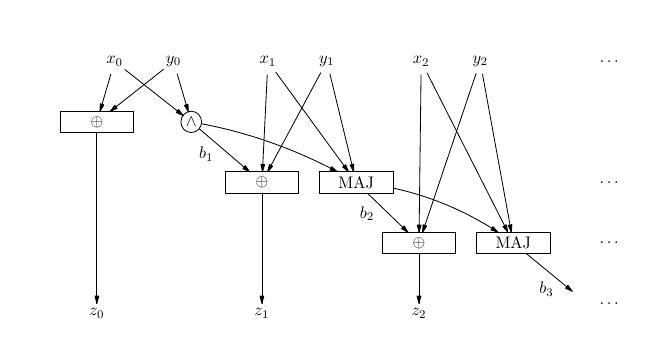
\includegraphics[]{img/schema}
        \end{center}

        Дальше, случай произвольных $z_i$ и $b_i$ полностью аналогичен случаю $z_1$ и $b_1$ и мы можем последовательно вычислить все эти значения.

        Оценим теперь размер описанной схемы. Для каждого разряда ответа нам нужно не больше двух раз применить подсхему для вычисления функции $\oplus$ и не более одного раза подсхему для вычисления $\MAJ_3$. Все эти схемы имеют фиксированный размер, так что для вычисления каждого разряда $z$ мы используем фиксированное число элементов, не зависящее от числа входных переменных. Поэтому всего в схеме $\O(n)$ элементов.

        \begin{problem*}
            Построим теперь схему для умножения $n$-битовых чисел. Пусть навход снова подаются два числа $x = \overline{x_{n - 1} \dots x_1 x_0}$ и $y = \overline{y_{n - 1} \dots y_1 y_0}$ . На этот раз мы хотим вычислить $z = x \cdot y$. Заметим, что $z$ имеет не больше $2n$ разрядов. Действительно, $x, y < 2^n$ , так что $z = x \cdot y \leq 2^{2n}$, а значит для его записи достаточно $2n$ разрядов.
        \end{problem*}

        Для вычисления $z$ снова воспользуемся школьным методом. В нем умножение двух чисел сводится к сложению n чисел. Действительно, чтобы умножить $x$ на $y$ достаточно для всякого $i = 0 \dots n - 1$ умножить $x$ на $y_i$, приписать в конце числа $i$ нулей и затем сложить все полученные числа. 
        
        Умножение $x$ на $y_i$ легко реализуется с помощью $n$ конъюнкций. Чтобы приписывать нули, их нужно иметь. В нашем определении не разрешается использовать константы. Поэтому нуль нужно вычислить. Для этого годится, например, такая схема:
        \begin{equation*}
            x_1 \land \neg x_1 = 0.
        \end{equation*}

        После этого остаётся сложить $n$ чисел длины не более $2n$. Для этого мы можем $n - 1$ раз применить схему для сложения, описанную выше. Размер каждой схемы для сложения линейный, так что суммарная сложность схемы для умножения получается $\O(n^2)$.

    \proofitem{Булева схема для задачи о связности графа. Оценка размера.}

        \begin{problem*}
            Дан неориентированный граф $G$ на $n$ вершинах. Нужно проверить, является ли он связным. Для этого удобно воспользоваться матрицей смежности графа. Перенумеруем вершины графа $v_1, v_2, \dots, v_n$. Матрицей смежности графа $G$ называется матрица $A \in \{0, 1\}^{n \times n}$, в которой на пересечении строки $i$ со столбцом $j$ стоит $1$ тогда и только тогда, когда в графе есть ребро $(v_i, v_j)$.
        \end{problem*}

        \begin{solution}
            Матрицу $A$ можно интерпретировать следующим образом: на пересечении строки $i$ и столбца $j$ написано количество путей длины $1$ из вершины $v_i$ в вершину $v_j$. Теперь возведём матрицу $A$ в квадрат (над действительными числами). Если посмотреть на формулу для произведения матриц можно заметить, что на пересечении строки $i$ и столбца $j$ матрицы $A^2$ записано количество путей длины $2$ из вершины $v_i$ в вершину $v_j$. По индукции можно доказать, что на пересечении строки $i$ и столбца $j$ матрицы $A^k$ записано число путей длины $k$ из вершины $v_i$ в вершину $v_j$. Заметим теперь, что если между какими-то двумя вершинами в графе есть путь, то обязательно есть путь длины не больше $n - 1$ (из пути всегда можно выкинуть циклы, если они там есть, после этого все вершины в пути разные). Так что для проверки связности у нас появляется такой план: вычислим все матрицы $A, A^2, \dots, A^{n - 1}$ и для каждой пары вершин $v_i$ и $v_j$ проверим, есть ли между ними путь длины не больше $n - 1$. Если это так, то граф связен, иначе не связен. 
            
            Этот план можно несколько упростить. Во-первых, можно немного модифицировать матрицу смежности. Рассмотрим матрицу $A'$, которая отличается от матрицы $A$ тем, что у неё на главной диагонали стоят единицы, а не нули (в остальном матрицы совпадают). В терминах графов это означает, что к каждой вершине мы добавляем петлю. В модели простых неориентированных графов мы этого не допускали, но ничего не мешает нам рассмотреть графы с петлями. Идея состоит в том, что теперь, если между двумя вершинами есть путь длины меньше $n - 1$, то есть и путь длины ровно $n - 1$ (достаточно добавить к пути нужное количество петель). Так что теперь не обязательно смотреть на все степени матрицы смежности, достаточно взглянуть на $(A')^{n - 1}$. Если в ячейках этой матрицы нет нулей, то граф связен, иначе не связен.
            
            Второе упрощение связано со способом возведения матрицы в степень. Выше мы считали число путей и для этого нужно складывать и умножать целые числа. Чтобы делать это с помощью булевых схем, нам придётся использовать схемы для сложения и умножения. Чтобы оценить размер получившейся схемы, придётся оценивать величину возникающих в процессе вычислений целых чисел. От этих сложностей можно избавиться.

            Решение состоит в том, чтобы вместо умножения матриц над целыми числами воспользоваться так называемым булевым умножением матриц. В нем формулы для умножения матриц такие же, как и в обычном умножении, только вместо операции умножения используется конъюнкция, а вместо сложения --- дизъюнкция. Тогда по индукции можно доказать, что в (булевой) матрице $(A')^k$ на пересечении строки $i$ и столбца $j$ стоит $1$ тогда и только тогда, когда в графе есть путь из $v_i$ в $v_j$ длины не больше $k$.

            Теперь мы готовы описать схему для проверки графа на связность. На вход схема (по существу) получает матрицу смежности $A'$. Схема последовательно вычисляет булевы степени этой матрицы $(A')^2, \dots, (A')^{n - 1}$ . Затем схема вычисляет конъюнкцию всех ячеек матрицы $(A')^{n - 1}$ и подаёт её на выход.

            Оценим размер получившийся схемы. Для булева умножения двух булевых матриц $n \times n$ достаточно $n^2 \cdot \O(n) = \O(n^3)$ операций (каждая ячейка произведения матриц вычисляется за линейное число операций, всего ячеек $n^2$). Всего нам нужно $(n - 1)$ умножение матриц, так что для вычисления матрицы $(A')^{n - 1}$ достаточно $\O(n^4)$ операций. На последний этап (конъюнкция ячеек $(A')^{n - 1}$ нужно $\O(n^2)$ операций, итого получается $\O(n^4) + \O(n^2) = \O(n^4)$ операций.
        \end{solution}

    \proofitem{Задача об угадывании числа. Верхняя и нижняя оценки.}

        Рассмотрим следующую игру. Алиса загадывает натуральное число от $1$ до $N$, а Боб пытается это число отгадать. При этом Бобу разрешается задавать вопросы, на которые Алиса может ответить <<да>> или <<нет>>, и Алиса должна на эти вопросы давать правильные ответы. Цель Боба состоит в том, чтобы задать как можно меньше вопросов.

        \begin{theorem*}
            Для угадывания числа от $1$ до $N$ необходимо и достаточно $\ceil{\log_2 N}$ вопросов.
        \end{theorem*}

        \begin{proof} \textbf{(Верхняя оценка)}

            Обозначим $k = \ceil{\log_2 N}$ и $N' = 2^k$. Видно, что $N' \geq N$. Пусть теперь Боб изначально считает, что Алиса может загадать число от $1$ до $N'$. Поскольку на самом деле Алиса может загадывать только числа от $1$ до $N$, то тем самым Боб только усложняет себе задачу и верхняя оценка не портится.

            Воспользуемся методом деления пополам. Идея в том, что Боб каждым своим вопросом будет сокращать количество оставшихся возможных чисел в два раза. Обозначим число, загаданное Алисой, через $x$. На каждом шаге Боб будет знать, что $x$ лежит в некотором отрезке $\{y \mid a \leq y \leq b\}$ для каких-то $a$ и $b$. Изначально $a = 1$ и $b = N'$. На очередном шаге Боб будет вычислять $c = \dfrac{a + b}{2}$ и спрашивать, верно ли, что $x \leq c$. 
            
            Если Алиса отвечает <<да>>, то Боб переходит к отрезку $\{y \mid a \leq y \leq c\}$ и повторяет процедуру. Иначе, Боб переходит к отрезку $\{y \mid c + 1 \leq y \leq b\}$ и также повторяет процедуру.

            На каждом шаге в каждом отрезке будет четное число точек и каждый отрезок будет делиться ровно пополам. Поэтому, чтобы длина отрезка стала равной $1$, потребуется ровно $\log_2 N' = k$ вопросов.
        \end{proof}

        \begin{proof} \textbf{(Нижняя оценка)} 

            Применим \textbf{мощностной метод}. Пусть у Боба есть какой-то алгоритм сложности $k$ (то есть, в нем всегда задается не более $k$ вопросов), Алиса загадала какое-то число и Боб задал свои вопросы. Рассмотрим цепочку ответов Алисы. Для удобства будем обозначать ответ <<да>> цифрой $1$, а ответ <<нет>> цифрой $0$. Тогда последовательность ответов Алисы --- это последовательность из $0$ и $1$ длины не больше $k$. 
            
            Заметим, что для двух разных загаданных Алисой чисел последовательности не могут совпадать. 
            
            Действительно, если для двух различных $x$ и $y$ Алиса дает Бобу на его вопросы полностью одинаковые ответы, то для Боба эти случаи неразличимы: его диалоги с Алисой для $x$ и для $y$ выглядят одинаково. При этом Боб после этого диалога выдает какой-то ответ, который определяется только состоявшимся диалогом. Значит в одном из случаев его ответ будет неправильным. 
            
            Далее, заметим, что не может быть так, что для двух различных $x$ и $y$, загаданных Алисой, цепочка ответов для $x$ является началом цепочки ответов для $y$.
            
            Действительно, иначе диалог Боба с Алисой выглядит одинаково для $x$ и $y$ до того момента, когда будут заданы все вопросы из цепочки ответов для $x$. Значит к этому моменту Боб не может отличить $x$ от $y$ и должен делать для них одно и то же, тогда как он в одном случае задает следующий вопрос, а в другом нет. Таким образом, мы получили, что каждому числу от $1$ до $N$ соответствует последовательность из не более чем $k$ нулей и единиц, все эти последовательности различны, и ни одна не является началом другой. 
            
            Заметим, что семейство этих последовательностей содержит не более $2^k$ элементов. 
            
            Действительно, если какая-то из них имеет длину меньше $k$, то продолжим ее, например, нулями. Тогда для различных $x$ и $y$ полученные последовательности длины $k$ различны: иначе они либо совпадают, либо одна (более короткая) является началом другой. 
            
            Таким образом, каждому числу от $1$ до $N$ соответствует последовательность длины $k$ из нулей и единиц, и все эти последовательности различны. 
            
            Всего последовательностей длины $k$ из нулей и единиц $2^k$. По принципу Дирихле, чисел от $1$ до $N$ должно быть не больше $2^k$ (иначе двум разным числам соответствуют одинаковые последовательности). Значит $N \leq 2^k$ , то есть $k \geq \log_2 N$. Поскольку $k$ --- целое число, то отсюда следует, что $k \geq \ceil{\log_2 N}$.
        \end{proof}


    \proofitem{Задача о сортировке нижняя оценка.}

        Дано $n$ объектов, все разного веса. За один шаг разрешается сравнить веса двух объектов (мы узнаем, какой из этих объектов тяжелее). Требуется расположить эти объекты в порядке возрастания веса.

        \begin{theorem*}
            Сложность задачи о сортировке $n$ объектов не меньше $\sum_{k = 1}^n \ceil{\log_2 k}$.
        \end{theorem*}

        \begin{proof}
            Доказательство будем вести индукцией по $n$. 
            
            Для $n = 1$ оценка верна --- никаких сравнений не требуется.

            Пусть утверждение доказано для $n$, докажем его для $n + 1$. Сначала возьмем первые $n$ объектов и упорядочим их, пользуясь предположением индукции. После этого у нас остается $\ceil{\log_2 (n + 1)}$ сравнений, и нам нужно один оставшийся объект поместить в уже упорядоченный список из $n$ объектов. То есть, для $(n + 1)$го объекта есть $n + 1$ место среди упорядоченного списка из $n$ объектов и нам нужно его найти. Пользуясь тем же рассуждением, что и в задаче про угадывание числа, это можно сделать как раз за $\ceil{\log_2 (n + 1)}$ сравнение (сравниваем со средним объектом и сокращаем количество возможных позиций почти в два раза).
        \end{proof}

    \proofitem{Задача о нахождении самой тяжелой монеты. Верхние и нижние оценки.}

        \begin{theorem*}
            Для нахождения самого тяжелого из $n$ объектов необходимо и достаточно $n - 1$ взвешивания.
        \end{theorem*}

        \begin{proof}~

            \begin{itemize}[leftmargin=*]
            \item
                Сначала докажем, что $n - 1$ взвешивания достаточно. Проще всего вести рассуждение по индукции. 
                
                Если $n = 1$, то ничего взвешивать не нужно. 
                
                Пусть мы доказали утверждение для $n - 1$. Рассмотрим $n$ объектов. Возьмем любые два и сравним их. Заметим, что более легкий из них не может быть самым тяжелым, так что его можно выбросить из рассмотрения. Таким образом у нас остается $n - 1$ объект и по предположению индукции мы можем найти самый тяжелый из них за $n - 2$ оставшихся взвешивания.

            \item
                Теперь докажем, что меньше чем за $n - 1$ взвешивание найти самый тяжелый объект нельзя. Пусть мы сделали $n - 2$ взвешивания. Рассмотрим следующий граф.
                
                Его вершинами будут наши объекты, и мы соединяем ребрами те из них, которые мы сравнили в одном из взвешиваний. Тогда в этом графе $n$ вершин и $n - 2$ ребра. Значит этот граф не связен. 
                
                Рассмотрим множество $V_1$ объектов в одной из его компонент связности и множество $V_2$ всех остальных объектов. Предположим, для определен ности, что самый тяжелый объект находится в $V_1$. Увеличим вес всех объектов в $V_2$ на одно и то же очень большое число, такое чтобы все объекты в $V_2$ стали тяжелее всех объектов в $V_1$. При этом результаты всех взвешиваний не изменятся, поскольку все сравнения были либо внутри $V_1$, либо внутри $V_2$, а самая тяжелая монета станет другой (теперь она будет в $V_2$). 
                
                Таким образом, все взвешивания дадут один и тот же результат в обеих ситуациях, а самый тяжелый объект будет разным. Значит в одной из двух ситуаций наш протокол выдает неправильный ответ. Мы пришли к противоречию, а значит для нахождения самого тяжелого объекта требуется не меньше $n - 1$ сравнения.
            \end{itemize}
        \end{proof}

    \end{colloq}

\end{document}